%!TEX root = ../main.tex
\subsection*{Responses to Reviewer \#2}
\label{cover_letter:r2}

\begin{shaded}
{

\stitle{R2W1}: 
\emph{Most components of the proposed framework resemble existing agentic LLM frameworks.
}

\stitle{R2D1:}
\emph{The overall architecture combines several elements that are now common in recent LLM-based agentic systems: iterative plan–execute loops, execution feedback, structured search over candidate solutions, reinforcement learning training, and synthetic task generation. While the integration of these components for autonomous data preparation is interesting, the paper would benefit from a clearer description of which aspects represent new technical contributions. In particular, the authors should help the reader to understand more precisely what algorithmic insight or system capability distinguishes the proposed approach from existing agentic solutions.}

}
\end{shaded}

\noindent{\bf RESPONSE}:
We thank the reviewer for this important comment.
While \sys incorporates several techniques that have appeared in prior agentic systems, such as execution feedback, tree search, and reinforcement learning, its contribution is not a simple combination of existing components.
Autonomous data preparation (ADP) differs fundamentally from tasks such as code generation and Text-to-SQL: it requires reasoning over evolving table states and multi-step data transformations. To address these challenges, \sys introduces a reasoning framework and training methods specifically designed for ADP.

Specifically, the novelty of \sys lies in two aspects.

\stitle{(1) Tree-based Agentic Reasoning for ADP.}
We introduce Tree-based Agentic Reasoning, a structured reasoning mechanism for multi-step data preparation. 
We further compare the mechanism with existing solutions to highlight its novelty.
Unlike ReAct~\cite{yao2023react}, \sys maintains explicit table states and supports rollback to previously valid states. Unlike Tree-of-Thought~\cite{yao2023tree}, exploration is grounded in executable data transformations and execution feedback. Unlike MCTS-based approaches~\cite{li2025alphasql}, the search process is represented as an explicit reasoning tree that can be serialized into prompts, enabling global reasoning over both successful and failed exploration trajectories.

\stitle{(2) Progressive Agentic Training for ADP.}
Existing agentic systems are primarily designed for inference-time exploration and are not explicitly trained to follow a structured reasoning protocol. To address this gap, \sys introduces Progressive Agentic Training, which trains the model to perform Tree-based Agentic Reasoning through control-tag supervision, execution-aware optimization, and a hybrid reward that combines outcome, partial, and process rewards. This enables effective multi-turn reasoning and exploration for ADP tasks. Moreover, \sys introduces a verification-in-the-loop mechanism to construct training data tailored for ADP tasks. Unlike standard data augmentation that applies random perturbations without guaranteeing solvability, \sys injects noise using inverse operators of data-cleaning functions (e.g., the inverse of date-standardization converts normalized dates into heterogeneous formats), and verifies reversibility by applying the corresponding cleaning operator to ensure the previous table state is restored. This guarantees that every synthesized task has a valid pipeline solution, which random noise injection cannot ensure.
% \fanj{Check the above paragraph. You should focus on the key \textbf{differences}, instead of technical details.}

%Second, \sys proposes a novel Progressive Agentic Training tailored for our Tree-based Agentic Reasoning method. Specifically, it conduct cold-start to train the agent to use the pre-defined control tags in Tree-based Agentic Reasoning, i.e., \action{plan}, \action{expand}, \action{execute} and \action{answer}. Moreover, considering that not all tokens should be considered during gradients optimization, we mask the tokens in the \action{execute} tag. At last, we design a hybrid reward for multi-turn RL training tailored for ADP scenarios, which is not covered by previous method. We integrates Outcome Reward calculated by the matching results of generated table and ground-truth target table, Partial Reward calculated by the similarity of generated table and ground-truth target table and Process Reward defined as reasoning process quality, together to provide dense learning signals.

{
To address the reviewer's concern, we have added a new paragraph, i.e., \textbf{Differences from existing agentic solutions}, in the \textbf{Introduction} (Section~\ref{sec:intro}) to more clearly distinguish the technical contributions of \sys from existing agentic frameworks.
}

% We appreciate this observation. While plan-execute loops, RL, and data synthesis are indeed common building blocks, the novelty of \sys lies in the technical innovations within each component and their co-design, which are necessary to make tree-based agentic reasoning work for ADP.

% \stitle{Inference.} The innovation of inference module is our propsosed Agentic Tree-based Reasoning module.
% Existing tree-search methods operate over text or latent space. Tree-of-Thoughts~\cite{yao2023tree} evaluates candidate reasoning steps as text, and MCTS-based agents~\cite{ge2025monteprep, li2025alphasql} rely on rollout-based value estimates and scalar reward signals to guide node selection and backpropagation. However, data preparation pipelines expose structured execution feedback, such as schema mismatches, execution errors, and intermediate table states. Such execution-level signals can not be captured by scalar rollout statistics. In contrast, \sys introduces an agentic reasoning tree that \emph{materializes execution states} (intermediate tables) at each node and makes branch decisions based on structured execution feedback rather than scalar rewards. This enables precise state recovery. The agent can backtrack to any prior node and branch from its exact table state, rather than re-generating from scratch. Furthermore, we \emph{preserve} failure states with their error traces and serialize them into prompts for subsequent reasoning, enabling failure-aware branching that prevents the agent from repeating the same mistakes (Section~\ref{subsec:agentic_tree_based_definition}, \action{execute} action).

% \stitle{Training.} The contribution in the training stage is the proposed Progressive Agentic Training with Environment Token Masking and Hybrid Reward.
% Standard SFT optimizes all tokens uniformly and standard GRPO/RLHF applies policy gradients over the entire output sequence. \sys introduces two technical innovations. First, \emph{environment token masking}. Since environment-generated tokens (execution results inside \action{execute} blocks) are deterministic outputs rather than policy decisions, we zero their gradients and optimize only agent decision tokens (\action{plan}, \action{expand}, \action{answer}). Second, a \emph{hybrid reward} with three components: (i) an outcome reward for strict correctness, (ii) a partial reward that measures table-level incremental progress via formal metrics (Jaccard similarity on column names, exponential shape penalty, cell-wise value matching), and (iii) a process reward where an LLM judge evaluates plan-action consistency, feedback responsiveness, and backtracking justification to discourage reward hacking.

% \stitle{Data.} 
% Standard data augmentation applies random perturbations without guaranteeing solvability. \sys injects noise by applying \emph{inverse operators} (e.g., the inverse of date-standardization produces heterogeneous formats), and after each corruption step, verifies reversibility by applying the corresponding cleaning operator to check that the previous table state is restored. Only verified corruptions are retained. This verification-in-the-loop mechanism guarantees that every synthesized task has a valid pipeline solution, which random noise injection cannot ensure.

\begin{shaded}
{
\stitle{R2W2}: 
\emph{Much of the evaluation uses datasets synthesized from NL2SQL benchmarks, which may not capture realistic data preparation challenges.
}

\stitle{R2D2}: 
\emph{A substantial portion of the experimental evaluation relies on datasets synthesized from NL2SQL benchmarks. While this strategy enables the generation of large datasets with long transformation pipelines, such synthetic tasks may not fully capture the complexity of real-world data preparation scenarios. In practice, data preparation often involves data quality issues that are difficult to reproduce through synthetic generation. I would suggest adding experiments on real-world datasets or practical case studies to strengthen the empirical evidence and provide a clearer picture of the system's applicability in realistic settings.
}
%
}
\end{shaded}

\noindent{\bf RESPONSE}:
We thank the reviewer for this valuable suggestion. To better evaluate the applicability of \sys in realistic settings, we have \textbf{added a new real-world dataset, Buildings~\cite{sharma2023automatic}, and conducted a new experiment (Exp-\ref{exp:building_exp}) on the dataset}.

%We have \textbf{added a new real-world dataset} Buildings~\cite{sharma2023automatic} and \textbf{conducted a new experiment (Exp-\ref{exp:building_exp})} on the new dataset. 

The Buildings dataset contains 105 real-world ADP tasks collected from data processing pipelines in the smart building domain across 21 energy companies. Specifically, it contains practical data quality issues commonly encountered in real-world data preparation. For example, column names are often abbreviated or domain-specific (e.g., ``\texttt{hdd}'', ``\texttt{cdd}''), and the same concept may be represented using different names across tables. These characteristics require semantic reasoning beyond schema matching and therefore provide a more realistic evaluation of autonomous data preparation systems.

%This dataset comprises 105 real-world ADP tasks collected from data processing pipelines in the smart building domain across 21 energy companies. It involves real-world data quality issues like ambiguous semantics. For example, in this dataset, column names are often abbreviated or domain-specific, e.g., hdd, cdd. Also, same concept may be represented by different names across tables. We evaluate on this Buildings dataset to provide a clearer picture of \sys's applicability in realistic settings.

We compare \sys with all ADP baselines in terms of accuracy, completion rate, and API cost. As reported in Table~\ref{\labelprefix tbl:buildings_exp}, \sys achieves the best overall performance. Specifically, it attains a 100\% completion rate and improves accuracy by 8.56 points over the second-best method. At the same time, its API cost remains relatively low compared with competing approaches. Therefore, consistent with the results on Synth-Spider, Synth-Bird, and Parrot, \sys achieves the best trade-off between accuracy and cost on this real-world dataset.

{We have revised \textbf{Section~\ref{subsec:exp-setup}} and \textbf{Section~\ref{subsec:in_depth_analysis}} to include the Buildings benchmark, experimental results, and analysis.} Moreover, we have added a practical case study to provide a clearer picture of the system’s applicability
in realistic settings, please refer to \textbf{Appendix~\ref{sec:appendix_case_study}} in our technical report~\cite{technical_report} for more details.

%We have compared \sys with ADP baselines over accuracy, complete rate and API cost. As reported in Table~\ref{\labelprefix tbl:buildings_exp}, \sys achieves the best performance among all methods. Specifically, it achieves 100\% complete rate and improves the accuracy of the second best methods by 8.56. Moreover, the api cost of \sys is relatively low. These experimental results demonstrate that \sys achieves the best best accuracy-cost trade-off on real-world dataset, as observed on Synth-Spider, Syth-Bird and Parrot.

% We appreciate this concern and have addressed it by \textbf{adding new experiments (Exp-\ref{exp:building_exp})}. We have evaluated \sys on a real-world ADP benchmark and conducted an error analysis to provide a clearer picture of \sys's applicability in realistic settings. Please refer to Response in \textbf{R1W3} and \textbf{R1D5} for detailed description.

\begin{shaded}
{
\stitle{R2W3}: 
\emph{The experimental setup provides limited information on prompt design and tuning for baseline methods.
}

\stitle{R2D3:}
\emph{The experimental setup includes several baseline methods, but the description of prompt design, parameter tuning, and configuration choices for these baselines is relatively limited. Since the performance of LLM-based baselines can depend heavily on prompt engineering and inference parameters, it is difficult to assess whether the comparisons are fair. The authors should provide more detailed information on how these baselines were implemented, which would make it easier to assess the fairness and reproducibility of the comparisons.}
}
\end{shaded}

\noindent{\bf RESPONSE}: 
We thank the reviewer for this important comment.
To ensure fair and reproducible comparisons, we apply a consistent configuration and tuning method across all baselines and provide the complete prompts, hyper-parameters, and implementation details in {our technical report~\cite{technical_report} (due to the space limit).}

Specifically, for methods with publicly available implementations, including MontePrep~\cite{ge2025monteprep}, DeepAnalyze~\cite{zhang2025deepanalyze}, AutoPrep~\cite{fan2024autoprep}, and MCTS-Op~\cite{li2025alphasql}, we use their official codebases and default configurations (e.g., prompt design, parameters, etc.). 
When a method was originally designed for a different task and could not be directly applied to ADP, we adapted its prompt to the ADP setting and tuned its parameters using the same grid-search procedure adopted by \sys. For example, AutoPrep was originally designed for TableQA rather than autonomous data preparation, so we replaced its original prompt with an ADP-oriented prompt and tuned it accordingly.

For methods without publicly available implementations, including CodeGen, ReAct, and PaS, we reimplemented them following the descriptions in their papers and applied the same prompt-tuning and parameter-selection procedure used for \sys. Therefore, all methods were evaluated under a comparable tuning method.

% \fanj{
% To improve reproducibility, we have added a detailed description of prompts, inference parameters, and configuration choices for all baselines in \textbf{Section~\ref{xxx}}. Complete prompts, hyper-parameters, and implementation details are also provided in our technical report~\cite{xxx}.
% }

To improve reproducibility, we have added the description of prompts, inference parameters, and configuration choices for all baselines in \textbf{Section~\ref{subsec:exp-setup}}. Complete prompts, hyperparameters, and implementation details are also provided \textbf{Appendix~\ref{sec:appendix_baselines}} in our technical report~\cite{technical_report}.

%For methods with published source codes, i.e., MontePrep~\cite{ge2025monteprep}, DeepAnalyze~\cite{zhang2025deepanalyze}, AutoPrep~\cite{fan2024autoprep} and MCTS-Op~\cite{li2025alphasql}, we directly use their public codes with default prompt, parameter and configuration choices. When some methods can not be directly adopted to our ADP scenario, we adopt greedy search to turn an optimized prompt for ADP tasks. For example, AutoPrep~\cite{fan2024autoprep} is first designed for TableQA task, we replace its original prompt with a well-tuned prompt for ADP tasks to support autonomous data preparation. For methods without published source codes, i.e., CodeGen, ReAct and PaS, we adopt greedy search same as \sys for their prompt design, parameter tuning, and configuration choices. The complete introduction of used prompts, hyper-parameters and configurations can be found in our technical report.

% As suggested, we have \textbf{added more critical information} for the implemented baselines, including hyper-parameters and prompt design. We provide a complete version of implementation details in our technical report~\cite{technical_report} due to space limit.
% We clarify the fairness of our comparisons from four aspects.

% (1) For methods with released source codes, e.g., MCTS-Op, MontePrep and DeepAnalyze, we directly follow the original implementation with default hyper-parameters.
% (2) All operator-assisted methods, including PaS, ReAct, MCTS-OP, AutoPrep and \sys, share the same operator space defined in Section~\ref{subsec:operator_space} and same execution environment. This ensures that performance differences stem from the reasoning strategy rather than the action space or execution backend.
% % \stitle{Consistent Hyper-Parameter.} 
% (3) We keep the hyper-parameters consistent across all methods whenever possible. Specifically, all prompting methods use the same temperature (0.01), and the same maximum input token limit (32k). 
% We set the maximum exploration turn to 5 for methods required to specify this hyper-parameter, involving \sys, CodeGen and DeepAnalyze.
% Training baselines (IL, RL-GRPO) use the same backbone models and hyper-parameter as \sys, differing only in the training strategy. This isolates the effect of our progressive agentic training.
% % \stitle{Consistent Prompt Design.} 
% (4) All methods share the same prompt structure, consisting of \texttt{Role}, \texttt{Demonstration}, and \texttt{Hint}. For operator-assisted method, it includes an additional part named \texttt{Operator Space}. We use same data preparation cases in the Demonstration section. 
% All methods shares the same serialization function and hyper-parameter (maximum column number and row number) for table serialization. 

\begin{shaded}
{
\stitle{R2W4}: 
\emph{The evaluation mainly reports inference cost but lacks a systematic analysis of scalability with respect to data size, schema complexity, or pipeline length.
}

\stitle{R2D4:}
\emph{The paper evaluates efficiency primarily through an inference cost metric based on runtime and GPU pricing. While this metric provides a useful indication of practical deployment cost, the evaluation does not include a systematic analysis of scalability.
In particular, it is not clear how the system behaves as input data size increases, as the number of tables grows, or as pipeline length and reasoning-tree exploration become more complex. Additional experiments analyzing runtime and resource usage under varying workload sizes would provide a clearer understanding of the scalability of the proposed approach and would strengthen the evaluation of the system expected for a VLDB paper.}
}
\end{shaded}



\begin{figure}[t]
    \centering
    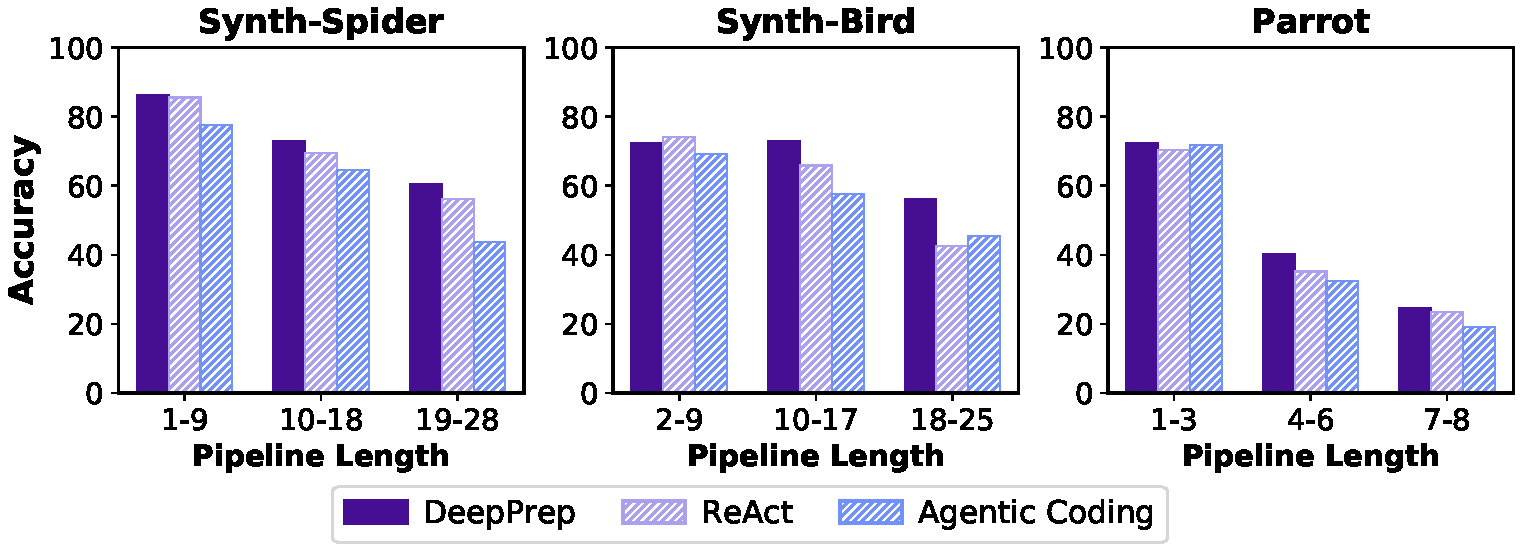
\includegraphics[width=1.01\columnwidth]{plots/plot/performance_compare_on_task_diff_claude.pdf}
    \vspace{-2em} 
    \caption{Comparison on Accuracy with varying Pipeline Length.}
    \label{\labelprefix fig:performance_compare_on_task_diff_claude}
    \vspace{-1em}
\end{figure}

\begin{figure}[t]
    \centering
    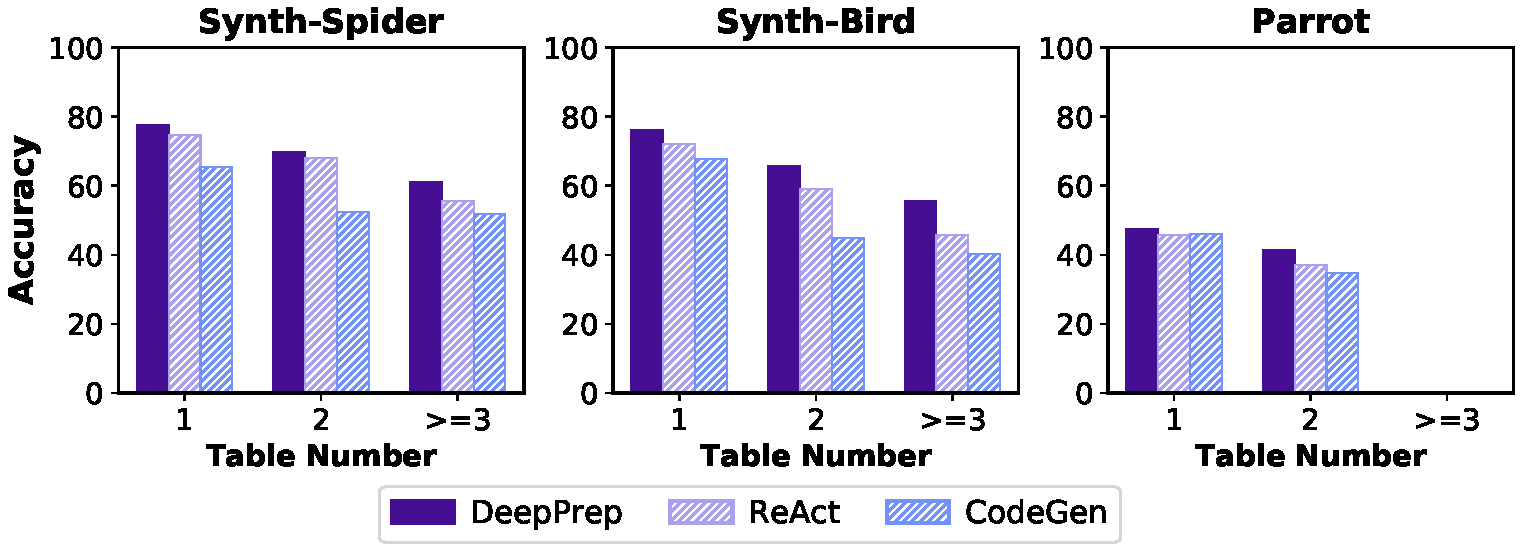
\includegraphics[width=1.01\columnwidth]{plots/plot/performance_compare_by_table_number_acc.pdf}
    \vspace{-2em} 
    \caption{Comparison on Accuracy with varying number of source tables.}
    \label{\labelprefix fig:performance_compare_by_table_number_acc}
    \vspace{-0.5em}
\end{figure}


\begin{table}[t]
  \centering
  \caption{\bf Average Execution Time (s) and Memory Usage (MB) under Varying Data and Task Complexity.}
  \vspace{-1em}
  \label{\labelprefix tbl:avg_time_memory_by_data_characteristics}
  \resizebox{0.99\columnwidth}{!}{
    \begin{tabular}{|c|c||c|c|c|c|c|c|}
      \hline
      \multirow{2}{*}{\textbf{Data Type}} 
      & \multirow{2}{*}{\textbf{Group}}
      & \multicolumn{2}{c|}{\textbf{Synth-Spider}}
      & \multicolumn{2}{c|}{\textbf{Synth-Bird}}
      & \multicolumn{2}{c|}{\textbf{Parrot}} \\
      \cline{3-8}
      & 
      & \textbf{Time} & \textbf{Mem.}
      & \textbf{Time} & \textbf{Mem.}
      & \textbf{Time} & \textbf{Mem.} \\
      \hline \hline

      \multirow{5}{*}{\shortstack{\textbf{Column}\\\textbf{Size}}}
      & b1
      & 8.91 & 66.31
      & 11.46 & 77.34
      & 7.09 & 114.42 \\
      \cline{2-8}

      & b2
      & 8.21 & 66.54
      & 12.13 & 74.07
      & 9.76 & 116.51 \\
      \cline{2-8}

      & b3
      & 8.48 & 67.07
      & 12.12 & 85.35
      & 11.49 & 125.12 \\
      \cline{2-8}

      & b4
      & 10.19 & 69.32
      & 12.88 & 83.31
      & 10.36 & 137.34 \\
      \cline{2-8}

      & b5
      & 11.30 & 68.37
      & 13.78 & 90.70
      & 11.36 & 143.35 \\
      \hline
      \hline

      \multirow{5}{*}{\shortstack{\textbf{Row}\\\textbf{Size}}}
      & b1
      & 7.87 & 65.69
      & 11.48 & 88.66
      & 9.54 & 124.43 \\
      \cline{2-8}

      & b2
      & 8.13 & 65.99
      & 11.36 & 74.92
      & 10.57 & 124.72 \\
      \cline{2-8}

      & b3
      & 9.30 & 66.78
      & 13.57 & 79.24
      & 9.07 & 120.89 \\
      \cline{2-8}

      & b4
      & 10.63 & 68.33
      & 12.64 & 80.00
      & 10.13 & 127.47 \\
      \cline{2-8}

      & b5
      & 11.72 & 71.30
      & 13.96 & 88.31
      & 10.77 & 135.00 \\
      \hline
      \hline

      \multirow{3}{*}{\shortstack{\textbf{Operator}\\\textbf{Length}}}
      & g1
      & 8.54 & 66.74
      & 11.26 & 80.08
      & 6.85 & 114.01 \\
      \cline{2-8}

      & g2
      & 12.75 & 70.30
      & 14.58 & 85.02
      & 11.06 & 130.69 \\
      \cline{2-8}

      & g3
      & 14.62 & 68.53
      & 14.01 & 81.92
      & 12.22 & 132.31 \\
      \hline
      \hline

      \multirow{3}{*}{\shortstack{\textbf{Table}\\\textbf{Number}}}
      & 1
      & 8.06 & 66.51
      & 9.94 & 79.00
      & 9.58 & 124.41 \\
      \cline{2-8}

      & 2
      & 10.54 & 68.82
      & 13.11 & 83.38
      & 10.81 & 128.74 \\
      \cline{2-8}

      & $\geq$3
      & 13.49 & 68.54
      & 14.92 & 81.08
      & -- & -- \\
      \hline
    \end{tabular}
  }
  \vspace{-1em}
\end{table}




\begin{algorithm}[t]
\small
\caption{\sys: Tree-Based Agentic Inference}
\label{alg:sys}
\begin{algorithmic}[1]
\Require Source tables $S$ and target schema $\Sigma^*$
\State Initialize $G_0 = (N, E)$ with $N=\{n_0\}$, \textcolor{blue}{$n_0 \leftarrow \mathcal{S}$}
\While{the agent does not use \action{answer}}
    \State \textcolor{blue}{$\psi_t \sim \Prob_{\text{LLM}}(\cdot \mid G_{t-1}, \Sigma^*, \psi_{<<t})$} \Comment{\action{plan}}
    \State \textcolor{blue}{$\mathcal{P}_t \sim \Prob_{\text{LLM}}(\cdot \mid G_{t-1}, \psi_t)$} \Comment{\action{expand} from chosen parent}
    \State $n_{\text{curr}} \leftarrow \text{parent node identified by } \psi_t$
    \For{each operator $o$ in $\mathcal{P}_t$}
        \State \textcolor{blue}{$\mathcal{T}_{\text{out}} \leftarrow o(n_{\text{curr}})$} \Comment{\textcolor{blue}{\action{execute} operator on current state}}
        \If{execution succeeds}
            \State $n_{\text{new}} \leftarrow \text{new node with state } \mathcal{T}_{\text{out}}$
            \State $N \leftarrow N \cup \{n_{\text{new}}\}$; $E \leftarrow E \cup \{(n_{\text{curr}} \xrightarrow{o} n_{\text{new}})\}$
            \State $n_{\text{curr}} \leftarrow n_{\text{new}}$
        \Else
            \State \textcolor{blue}{Annotate $n_{\text{curr}}$ with failure trace}
            \State \textbf{break} 
        \EndIf
    \EndFor
    \State $G_t \leftarrow (N, E)$
\EndWhile
\State $n_\text{leaf}\leftarrow \mathtt{select} (\cdot|S,\Sigma^*, G_t)$
\State $D^*\leftarrow n_\text{leaf}$
\State \Return $D^*$
\end{algorithmic}
\end{algorithm}

\noindent{\bf RESPONSE}: 
We thank the reviewer for this valuable suggestion. We have \textbf{added a new scalability study that evaluates \sys under varying row sizes, column sizes, pipeline lengths, and table numbers}. We further {report runtime and memory usage across different complexity groups} to provide a systematic understanding of the scalability of \sys.

\stitle{Time and Resource Usage.}
We group cases according to row size, column size, pipeline length, and table number, and report the average execution time and memory usage in Table~\ref{\labelprefix tbl:avg_time_memory_by_data_characteristics}. 
In particular, for row-size and column-size analyses, we sort all cases by the corresponding metric and divide them into five equal-width buckets $b_1 - b_5$ (detailed bucket ranges for each dataset will be reported later).
As shown in the table, \sys exhibits stable growth in both execution time and memory usage as workload complexity increases. For example, on Synth-Spider, the average execution time increases only from 8.91 to 11.30 seconds when moving from the smallest to the largest column-size bucket, while memory usage remains between 66 MB and 69 MB. Similar trends are observed on Synth-Bird and Parrot. These results indicate that \sys scales gracefully with increasing data size and task complexity.

\stitle{Why \sys Scales Stably.}
The stable scaling behavior can be explained by the generative search framework formalized in Algorithm~\ref{alg:sys}. At each step, the agent generates a \action{plan} $\psi_t$ (Line 3) and an \action{expand} action (Line 4), followed by the execution of the proposed operators (Line 7). The process is bounded by the maximum exploration turn $T$ and the maximum operator sequence length $L$ per expansion, yielding a worst-case complexity of $O(T \times L)$. Unlike classical tree-search methods such as MCTS, which explicitly expand and evaluate many candidate branches, \sys generates only one operator pipeline conditioned on the current tree state. The ``pruning'' is implicit in the LLM's decision-making: the agent observes failure traces and avoids revisiting failed branches, rather than enumerating all possible expansions. Consequently, the effective branching factor depends on the LLM's learned policy and remains bounded regardless of input size, which explains the stable growth in time and memory usage.

We have revised \textbf{Exp-\ref{exp:scalability} (Scalability Analysis)} of \textbf{Section~\ref{subsec:in_depth_analysis}} to include the above experiments and discussion. A complete version can be found in \textbf{Appendix~\ref{subsec:appendix_sensitivity_data_size}-\ref{subsec:appendix_pipeline_table}} in our technical report~\cite{technical_report}.

\etitle{Additional Experimental Details.}
For row-size and column-size analyses, we sort all cases by the corresponding metric and divide them into five equal-width buckets $b_1 - b_5$, as described below.
%
\begin{itemize}[leftmargin=*]
    \item \textbf{The Synth-Spider dataset.}
    \begin{itemize}
        \item Column buckets: $b_1$ (1-4), $b_2$ (5-7), $b_3$ (8-9), $b_4$ (10-14), $b_5$ (15-124,843).
        \item Row buckets: $b_1$ (1-9), $b_2$ (10-15), $b_3$ (16-21), $b_4$ (22-35), $b_5$ (36-124,842).
    \end{itemize}
    \item \textbf{The Synth-Bird dataset.}
    \begin{itemize}
        \item Column buckets: $b_1$ (1-11), $b_2$ (12-27), $b_3$ (29-74), $b_4$ (75-1,003), $b_5$ (1,004-20,015).
        \item Row buckets: $b_1$ (1-110), $b_2$ (115-1,000), $b_3$ (1,001-1,022), $b_4$ (1,023-2,004), $b_5$ (2,005-360,006).
    \end{itemize}
    \item \textbf{The Parrot dataset.}
    \begin{itemize}
        \item Column buckets: $b_1$ (2-4), $b_2$ (5-7), $b_3$ (8-11), $b_4$ (12-16), $b_5$ (18-587).
        \item Row buckets: $b_1$ (2-13), $b_2$ (14-30), $b_3$ (31-100), $b_4$ (107-2,000), $b_5$ (2,075-200,000).
    \end{itemize}
\end{itemize}


%As suggested, we have added a systematic analysis of scalability with respect to column size, row size, pipeline length and table number. We group cases based on varying data characteristics and report the time and CPU memory usage in Table~\ref{\labelprefix tbl:avg_time_memory_by_data_characteristics}.
%
%\stitle{Accuracy under Varying Data Sizes.}
%We sort all cases by the number of columns and rows respectively, and divide them into five equal-width buckets ($b_1$ to $b_5$). As shown in Figures~\ref{\labelprefix fig:performance_compare_by_column_size_acc} and \ref{\labelprefix fig:performance_compare_by_row_size_acc}, \sys remains robust on small and medium-sized tables. Performance degrades only for the largest buckets. For cases in $b_5$, accuracy decreases by 29.54 points compared with cases in $b_1$. This degradation is primarily caused by the table sampling strategy used to control token consumption, where relevant information may be omitted from the sampled content for very large tables.
%
%\stitle{Accuracy under Varying Pipeline Length and Table Number.}
%For pipeline length, we partition ADP cases into Simple, Medium, and Complex groups according to the number of operators in the target pipeline. As shown in Figure~\ref{\labelprefix fig:performance_compare_on_task_diff_claude}, all methods degrade as the pipeline length increases. However, \sys shows the smallest degradation, and its advantage over baselines becomes larger on Complex cases. On Synth-Spider, \sys achieves 60.5 accuracy on Complex cases, outperforming Code Agent by 16.8 points. For table number, as shown in Figure~\ref{\labelprefix fig:performance_compare_by_table_number_acc}, performance generally decreases as more source tables are involved, but \sys consistently achieves the highest accuracy across different table number groups.
%
%\stitle{Time and Resource Usage.}
%As recorded in Table~\ref{\labelprefix tbl:avg_time_memory_by_data_characteristics}, both time and memory usage remain stable as data size increases. For example, on Synth-Spider, the average execution time increases only from 8.91 to 11.30 seconds when moving from the smallest to the largest column-size bucket, while memory usage remains between 66 MB and 69 MB. Similar trends are observed on Synth-Bird and Parrot.
%
%\stitle{Why \sys Scales Stably.}
%The stable scaling behavior can be explained by the generative search framework formalized in Algorithm~\ref{alg:sys}. At each step, the agent generates a \action{plan} $\psi_t$ (Line 3) and an \action{expand} action (Line 4), then physically executes the proposed operators (Line 7). This process is bounded by the maximum exploration turns $T$ and the maximum operator sequence length per expansion $L$, yielding a worst-case complexity of $O(T \times L)$. Unlike classical tree search methods such as MCTS that expand all candidate branches and perform rollout simulations for value estimation, \sys generates only one operator pipeline per step conditioned on the current tree state. The ``pruning'' is implicit in the LLM's decision-making: the agent observes failure traces and avoids revisiting failed branches, rather than enumerating all possible expansions. Consequently, the effective branching factor depends on the LLM's learned policy and remains bounded regardless of input size, which explains the stable growth in time and memory usage.